\documentclass[12pt]{beamer}

\usetheme{Malmoe}
\usepackage[utf8]{inputenc}
\usepackage{graphicx}
\usepackage{xcolor}
\usepackage{wrapfig} % texlive-latex-extra package
\usepackage{underscore}
\usepackage{listings}

\definecolor{Cyan}{RGB}{0,141,184}
\definecolor{codeblock}{RGB}{220,220,220}

\setbeamercolor{structure}{fg=Cyan}

\setbeamerfont{title}{series=\bfseries,parent=structure}
\setbeamerfont{subtitle}{size=\normalsize,series=\bfseries,parent=structure}
\setbeamerfont{author}{size=\scriptsize,series=\bfseries,parent=structure}
\setbeamerfont{institute}{size=\scriptsize,series=\bfseries,parent=structure}
\setbeamerfont{date}{size=\scriptsize,series=\bfseries,parent=structure}

%\ shell code block style (https://en.wikibooks.org/wiki/LaTeX/Source_Code_Listings)
\lstset{language=sh,
	basicstyle=\ttfamily\scriptsize,
	backgroundcolor=\color{codeblock},
	commentstyle=\color{blue},
	breaklines=true
}

\title{GIS.lab}
\subtitle{news from development of technology for rapid deployment of complete geospatial infrastructure with supercow capabilities}
\author{Ivan Minčík (imincik)}
%\setbeamercovered{transparent} 
%\setbeamertemplate{navigation symbols}{} 
%\logo{} 
\institute{FOSS4G Europe 2015, Como, Italy}
\date{} 
%\subject{}


% document BEGIN
\begin{document}


\begin{frame}
	\titlepage
\end{frame}

\begin{frame}{The Super Cow}
	\begin{center}
		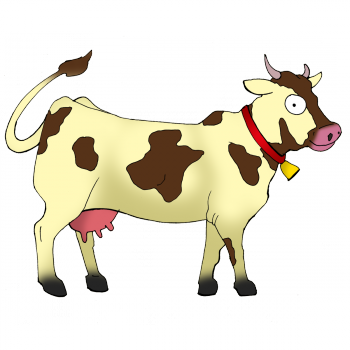
\includegraphics[keepaspectratio=true,height=0.6\textheight]{images/cow.png}
	\end{center}
\end{frame}


\section{Introduction}
\begin{frame}
	\begin{center}
		\LARGE\textbf{Introduction}	
	\end{center}
\end{frame}

\begin{frame}{The Problem}
	\begin{center}
		We always \textbf{need more than only one app} for our GIS work flow
	\end{center}
\end{frame}

\begin{frame}{The Problem}
	\begin{center}
		Deployment and maintenance of \textbf{complex system is hard} even if things are going flawlessly
		\end{center}
\end{frame}

\begin{frame}{The Problem}
	\begin{center}
		which usually they are \textbf{not} (:
	\end{center}
\end{frame}

\begin{frame}{GIS.lab}
	\textbf{Instantly} in production with \textbf{no feeding} !
	\begin{center}
		%\ image: cow with QGIS, GRASS and PostGIS in bottles
		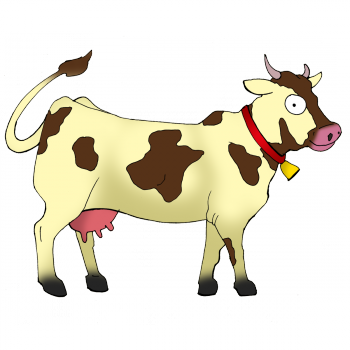
\includegraphics[keepaspectratio=true,height=0.6\textheight]{images/cow.png}
	\end{center}
\end{frame}


\section{What is GIS.lab ?}
\begin{frame}
	\begin{center}
		\LARGE\textbf{What is GIS.lab ?}
	\end{center}
\end{frame}

\begin{frame}{What is GIS.lab ?}
	\textbf{free} technology which can \textbf{instantly} turn pile of metal scrap in to the \textbf{high-end geospatial cluster}
	\begin{center}
		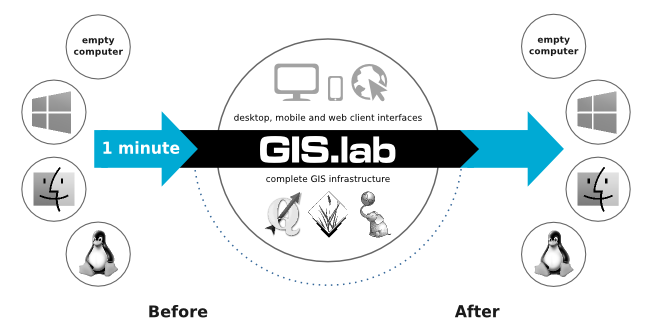
\includegraphics[keepaspectratio=true,height=0.5\textheight]{images/gislab-schema.png}
	\end{center}
\end{frame}

\begin{frame}{What is GIS.lab ?}
	\begin{center}
		and back to \textbf{the same scrap} again
	\end{center}
\end{frame}

\begin{frame}{Features}
	\begin{itemize}[<+->]
		\item so simple \textbf{plug-and-play} deployment as home router
		\item \textbf{central management}
		\item \textbf{desktop, web and mobile} client interfaces
		\item automatic \textbf{clustering and resources sharing}
		\item collaboration tools
		\item fits in your pocket \textbf{pocket}
		\item or \textbf{LAN, data center} and \textbf{cloud}
	\end{itemize}
\end{frame}

\begin{frame}{GIS.lab Architecture}
	\begin{center}
		%\ image: schema server and clients
		
\includegraphics[keepaspectratio=true,height=0.5\textheight]{images/image.png}
	\end{center}
\end{frame}

\begin{frame}{GIS.lab Server}
	\begin{center}
		%\ image: schema storage and management (gears)
		
\includegraphics[keepaspectratio=true,height=0.5\textheight]{images/image.png}
	\end{center}
	\begin{itemize}
		\item automatically installed
		\item data storage
		\item client launch support
		\item OWS load balancing
		\item central management
	\end{itemize}
\end{frame}

\begin{frame}{GIS.lab Clients}
	\begin{center}
		%\image: desktop + web + mobile
		
\includegraphics[keepaspectratio=true,height=0.5\textheight]{images/image.png}
	\end{center}
	\begin{itemize}
		\item launched from GIS.lab Server 
		\item user interfaces for data processing, analysis and collaboration
		\item computing power for GIS.lab Cluster
	\end{itemize}
\end{frame}


\section{What is new ?}
\begin{frame}
	\begin{center}
		\LARGE\textbf{So, what's new ?}	
	\end{center}
\end{frame}

\begin{frame}
	\begin{center}
		mostly \textbf{everything}
	\end{center}
\end{frame}


\section{Deployment}
\begin{frame}
	\begin{center}
		\LARGE\textbf{Deployment}	
	\end{center}
\end{frame}

\begin{frame}[fragile]{Automatic provisioning}
	\begin{center}
		
\includegraphics[keepaspectratio=true,height=0.4\textheight]{images/ansible.png}
	\end{center}

   \lstset{language=sh}
	\begin{lstlisting}
		$ ansible-playbook
		  --inventory=gislab.inventory
		  --private-key=~/.ssh/id_rsa
		  system/gislab.yml
	\end{lstlisting}
\end{frame}

\begin{frame}[fragile]{Development, testing, evaluation - virtual machine}
	\begin{center}
		
\includegraphics[keepaspectratio=true,height=0.4\textheight]{images/vagrant.png}
		
\includegraphics[keepaspectratio=true,height=0.4\textheight]{images/virtualbox.png}
		
\includegraphics[keepaspectratio=true,height=0.4\textheight]{images/ansible.png}
	\end{center}

   \lstset{language=sh}
	\begin{lstlisting}
		$ vagrant up
		Bringing machine 'gislab_vagrant' up with 'virtualbox' provider...
		==> gislab_vagrant: Importing base box 'precise-canonical'...
		==> gislab_vagrant: Running provisioner: install (ansible)...
	\end{lstlisting}
\end{frame}

\begin{frame}{End User Deployment - GIS.lab Unit}
	\begin{center}
		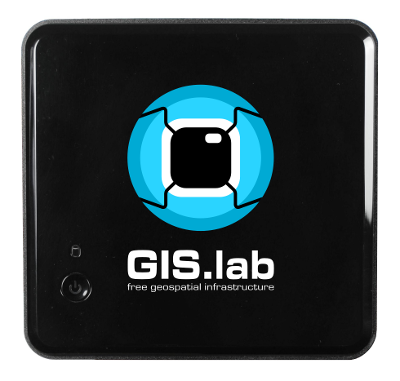
\includegraphics[keepaspectratio=true,height=0.6\textheight]{images/gislab-unit.png}
	\end{center}
	\begin{itemize}
		\item portable, pocket size
		\item plug-and-play
		\item automatic adaptation to host network
	\end{itemize}
\end{frame}


\section{Client Interfaces}
\begin{frame}
	\begin{center}
		\LARGE\textbf{Desktop Client}	
	\end{center}
\end{frame}

\begin{frame}{Machines Launch}
	\begin{center}
		%\ image: boot from server - physical client and virtual one
		
\includegraphics[keepaspectratio=true,height=0.5\textheight]{images/image.png}
	\end{center}
	\begin{itemize}
		\item network launch (PXE, HTTP)
		\item physical hardware or virtual client mode
		\item working with every network configuration
	\end{itemize}
\end{frame}

\begin{frame}{Desktop Client}
	\begin{center}
		%\ image: desktop client screenshot with QGIS, GRASS ...
		
\includegraphics[keepaspectratio=true,height=0.5\textheight]{images/image.png}
	\end{center}
	\begin{itemize}
		\item QGIS as the geospatial project IDE
		\item integrated with GRASS 7 and others
	\end{itemize}
\end{frame}

\begin{frame}{Maps Publishing on Web}
	\begin{center}
		%\ image: gis.lab web plugin
		
\includegraphics[keepaspectratio=true,height=0.5\textheight]{images/image.png}
	\end{center}
	\begin{itemize}
		\item publish any QGIS project with GIS.lab Web QGIS
	\end{itemize}
\end{frame}

\begin{frame}[fragile]{Customization}
	%\ own client image build system (replacing LTSP)
	\begin{itemize}
		\item customization in isolated environment using standard tools
		\item central image distribution
		\item rollback
	\end{itemize}
	
	\lstset{language=sh}
	\begin{lstlisting}
		$ cp /opt/gislab/client-desktop                  # backup
		     /mnt/backup/client-desktop.backup
		
		$ gislab-client-shell -i   # enter client env
		$ apt-get install gedit    # install Gedit
		$ exit                     # exit client env
		$ gislab-client-image      # deploy updated client image
		
		$ rm -rf /opt/gislab/client-desktop
		  &&
		  mv /mnt/backup/client-desktop.backup
		     /opt/gislab/client-desktop                  # rollback
	\end{lstlisting}
\end{frame}


\begin{frame}
	\begin{center}
		\LARGE\textbf{Web and Mobile Client}	
	\end{center}
\end{frame}

\begin{frame}{Web and Mobile Client}
	\begin{center}
		%\ image: web and mobile client screenshots
		
\includegraphics[keepaspectratio=true,height=0.5\textheight]{images/image.png}
	\end{center}
\end{frame}


\section{GIS.lab Cluster}
\begin{frame}
	\begin{center}
		\LARGE\textbf{GIS.lab Cluster}	
	\end{center}
\end{frame}

\begin{frame}{Automatic clustering}
	\begin{center}
		
\includegraphics[keepaspectratio=true,height=0.5\textheight]{images/serf.png}
	\end{center}
	\begin{itemize}
		\item decentralized cluster membership and failure detection system based on GOSSIP protocol
	\end{itemize}
\end{frame}

\begin{frame}[fragile]{Cluster management}
	\begin{itemize}
		\item based on cluster events, queries tags
	\end{itemize}

	\lstset{language=sh}
	\begin{lstlisting}
		$ gislab-cluster members
		$ gislab-cluster event <EVENT-NAME>
		$ gislab-cluster query <QUERY-NAME>		
	\end{lstlisting}

	\lstset{language=sh}
	\begin{lstlisting}
		$ gislab-cluster members
		server.gis.lab  192.168.15.5:7946 
		                alive  role=server

		c50             192.168.15.50:7946
		                alive
		                role=client,worker=yes,session-active=user1

		c51             192.168.15.51:7946
		                left
		                role=client,worker=yes
	\end{lstlisting}
\end{frame}


%\ clustering and management, Serf, decentralized GOSSIP. failure detection, events, queries 
%\ OWS load ballancing
%\ parallel computing


\section{Other}
\begin{frame}
	\begin{center}
		\LARGE\textbf{Other}
	\end{center}
\end{frame}

%\ Intergation tests
\begin{frame}{Tests}
\end{frame}

%\web - themes, raster and vector layers, drawings, sharing ... OL3, WPS
%\mobile

%\ resources sharing, clustering, pssh
%\ authors
%\ Amazon


% document END
\end{document}